\documentclass[11pt]{article}
\usepackage[main=polish,english]{babel}
\usepackage[utf8]{inputenc}
\usepackage[T1]{fontenc}
\usepackage[hidelinks]{hyperref}
\usepackage{xcolor}
\usepackage{enumitem}
\usepackage[a4paper,inner=3.5cm,outer=2.5cm,top=2.5cm,bottom=2.5cm]{geometry}
\usepackage{newtxtext, newtxmath}
\usepackage{graphicx}
\usepackage[section]{placeins}
\usepackage{cleveref}


\setlist[itemize]{noitemsep}
\linespread{1.3} %interlinia 1.5
\setlength{\parindent}{1.25cm}

\crefname{figure}{}{}
\Crefname{figure}{}{}
\crefname{table}{}{}
\Crefname{table}{}{}
\crefname{section}{}{}
\Crefname{section}{}{}
\crefname{chapter}{}{}
\Crefname{chapter}{}{}

% the document is below

\title{Zastosowanie programowania ewolucyjnego w celu rozwiązania problemu
    komiwojażera}

\author{Maciej Wieczór-Retman, Kacper Stojek}

\date{} %leave blank

\begin{document}

\maketitle

\section{Wstęp}

Problem komiwojażera (ang. \textit{Traveling salesman problem}) jest problemem
minimalizacji, polegającym na odnalezieniu minimalnego cyklu Hamiltona w pełnym
grafie ważonym. Cykl Hamiltona to taki cykl w grafie, w którym każdy wierzchołek
grafu jest odwiedzony dokładnie raz. Czyli rozwiązaniem problemu komiwojażera
jest cykl o najmniejszej sumie wag krawędzi grafu. Liczba różnych cyklów
Hamiltona $H$ dla pełnego grafu nieskierowanego o $n$ wierzchołkach jest
wyrażana równaniem \cref{equ:n_cycles}.
\begin{equation}
    H = \frac{\left(n - 1\right)!}{2}
    \label{equ:n_cycles}
\end{equation}
Z uwagi na liczbę różnych cyklów, przeszukiwanie wszystkich rozwiązań jest
fizycznie niemożliwe dla większych grafów. Przykładowo stosunkowo mały graf o
stu wierzchołkach, daje w przybliżeniu $4,7 \times  10^{155}$ rozwiązań. Dla
przybliżenia zakładając, że sprawdzenie jednej ścieżki zajmuje $1 \, \mu s$,
przeanalizowanie wszystkich ścieżek zajęłoby $1,48 \times  10^{142} \, lat$.
Z tego powodu ważne jest zastosowanie bardziej skomplikowanych algorytmów
minimalizacyjnych, takich jak właśnie programowanie genetyczne. Dobrze
skonstruowany algorytm powinien być w stanie znaleźć minimum globalne dla
większości przypadków lub przynajmniej optymalne rozwiązanie.

Napisany algorytm będzie testowany na danych z
{\color{blue} \href{https://www.math.uwaterloo.ca/tsp/vlsi/index.html}
{www.math.uwaterloo.ca}} w celu weryfikacji jego działania.

\section{Implementacja}

Jak zostało wspomniane na wstępie, rozwiązaniem problemu komiwojażera jest
najkrótszy cykl Hamiltona dla danego pełnego, ważonego i nieskierowanego grafu.
Z tych informacji wynikają szczegóły implementacji takie jak funkcja
przystosowania, reprezentacja osobników oraz ograniczenia co do sposobu mutacji,
oraz krzyżowania osobników.

Ponieważ szukany jest cykl Hamiltona, w rozwiązaniu
każdy wierzchołek grafu pojawi się tylko raz, to znaczy, że mając graf $G$ o $N$
wierzchołkach:
\begin{equation}
    V\left(G\right) = \left\{ v_1 \, v_2 \, \cdots v_N \right\},
\end{equation}
rozwiązaniem będzie pewna permutacja zbioru $V\left(G\right)$. Z uwagi na to,
najłatwiej jest wykorzystać kodowanie całkowitoliczbowe. Z tym kodowaniem każdy
wierzchołek dostaje swój indeks, a następnie każdy osobnik składa się z pewnej
permutacji wierzchołków grafu, reprezentując pojedynczy cykl Hamiltona.

Mając zdefiniowany sposób zapisu osobników, można w oparciu o to zdefiniować
funkcję przystosowania $f \left( x \right)$ dla osobnika $x$. Najpierw jednak
należy zdefiniować funkcję kosztu $u \left( x \right)$. Ponieważ pojedynczy
osobnik składa się z kolejnych indeksów wierzchołków, funkcją kosztu jest
suma wag krawędzi pomiędzy kolejnymi wierzchołkami, oraz dodatkowo pomiędzy
pierwszym a ostatnim wierzchołkiem w osobniku (szukany jest cykl grafu).
Następnie funkcja przystosowania $f \left( x \right)$ jest następująca:
\begin{equation}
    f \left( x \right) = C_{max} - u \left( x \right),
\end{equation}
gdzie:
\begin{itemize}
    \item[] $f \left( x \right)$ - funkcja przystosowania,
    \item[] $u \left( x \right)$ - funkcja kosztu,
    \item[] $C_{max}$ - parametr nie mniejszy niż maksymalna wartość
            $u \left( x \right)$ dla danej aktualnej populacji,
    \item[] $x$ - osobnik.
\end{itemize}

Z uwagi na naturę rozwiązania, metody krzyżowania osobników są ograniczone,
ponieważ allele w nowopowstałym osobniku nie mogą się powtarzać. Dlatego
przykładowo krzyżowanie arytmetycznie się nie nadaje. Możliwe sposoby
krzyżowania to:
\begin{itemize}
    \item PMX,
    \item OX,
    \item CX.
\end{itemize}
W projekcie użyto krzyżowania OX, ponieważ ta metoda krzyżowania najbardziej
zachowuje kolejność alleli w osobniku. Zamysł jest taki, aby osobniki wymieniały
się krótkimi trasami, zachowując ich kolejność. Dany osobnik na początku
działania algorytmu będzie miał zoptymalizowany tylko fragment trasy. Krzyżując
dwa osobniki, jest spora szansa, że ten fragment się zachowa i trafi do
kolejnego osobnika. Za mieszanie kolejności raczej powinny być odpowiedzialne
mutacje osobników. Metody krzyżowania PMX oraz OX za bardzo zmieniają szyk
alleli, przez co nie zostały wykorzystane.

Podobnie jak w przypadku krzyżowania, osobniki po mutacji dalej muszą tworzyć
poprawny ciąg Hamiltona. Z tego powodu mutacje ograniczają się do podmian
elementów w strukturze osobnika, bez zmian ich wartości. Dopuszczalne sposoby
mutacji to:
\begin{itemize}
    \item inwersja (ang. inversion),
    \item wstawianie (ang. insertion),
    \item przenoszenie (ang. displacement),
    \item wzajemna wymiana (ang. reciprocal exchange).
\end{itemize}
W projekcie użyto inwersji oraz wstawiania. Przy mutacji, szczególnie w
początkowej fazie działania algorytmu, ważne jest, aby mutacje miały charakter
globalny. Inwersja polega na wylosowaniu podciągu w osobniku i odwrócenie w nim
kolejności alleli, natomiast wstawianie polega na wylosowaniu pojedynczego
allela, i wstawienie go w innym, losowo wybranym miejscu. Wstawianie pozwala na
stworzenie nowych tras w osobnikach, tak zmiany są małe i algorytm przy tylko
takim rodzaju mutacji, szybko się zbiega do minimum lokalnego. Dlatego, aby
troch zwiększyć szansę na znalezienie innego, lepszego minimum, została dodana
inwersja. Ponieważ zmiany przy inwersji są bardziej drastyczne, jest większa
szansa, że populacja nie utknie od razu w minimum lokalnym. To czy zostanie
wykonana inwersja czy wstawianie też zależy od obecnej iteracji. Im wyższa
iteracja, tym większa szansa, że zostanie wykonane wstawianie zamiast inwersji.

Przy tworzeniu nowych osobników również trzeba uważać, aby nie tworzyć elity.
Zostawianie i krzyżowanie tylko najlepszych osobników, prowadzi do
przedwczesnego zbiegania się algorytmu do nieoptymalnego rozwiązania. Dlatego
osobniki są niszowane w ten sposób, że osobniki z gorszym przystosowaniu mają
większą szansę na trafienie do puli rodzicielskiej. W odwrotnej konfiguracji,
gdzie lepsze osobniki miały większą szansę na trafienie do puli rodzicielskiej,
algorytm przedwcześnie się zbiegał do suboptymlanego rozwiązania. Następnie po
przeprowadzeniu krzyżowania i wyznaczeniu nowych osobników, są one poddawane
mutacji. Po krzyżowaniu oraz mutacji są pozostawiani rodzice lub potomkowie, w
zależności od tego, który osobnik jest lepszy.

\section{Wyniki pracy}

Jak wspomniano na wstępie, algorytm został przetestowany na danych z
{\color{blue} \href{https://www.math.uwaterloo.ca/tsp/vlsi/index.html}
{www.math.uwaterloo.ca}} w celu weryfikacji jego działania. Pierwszym testowym
grafem jest
{\color{blue} \href{https://www.math.uwaterloo.ca/tsp/vlsi/xqf131.points.html}
{xqf131}}, którego wierzchołki są przedstawione na rysunku \cref{fig:xqf131}.
Natomiast drugim grafem testowym jest
{\color{blue} \href{https://www.math.uwaterloo.ca/tsp/vlsi/xqg237.points.html}
{xqg237}}, którego wierzchołki są przedstawione na rysunku \cref{fig:xqg237}.
\begin{figure}
    \centering
    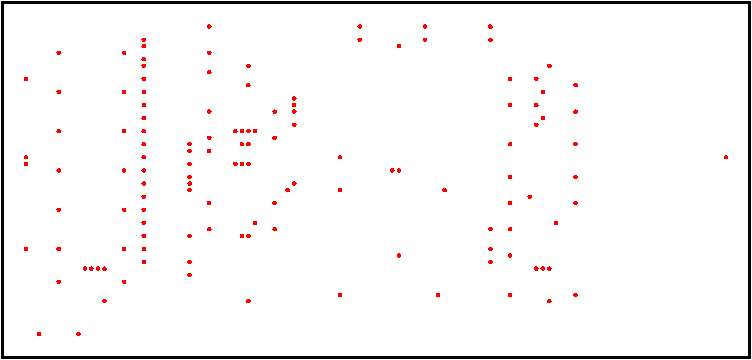
\includegraphics[scale=0.7]{img/xqf131.png}
    \caption{Wierzchołki grafu xqf131}
    \label{fig:xqf131}
\end{figure}
\begin{figure}
    \centering
    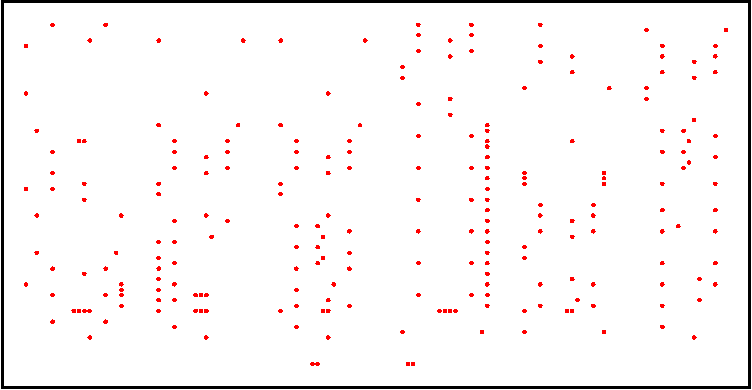
\includegraphics[scale=0.7]{img/xqg237.png}
    \caption{Wierzchołki grafu xqg237}
    \label{fig:xqg237}
\end{figure}

Początkowo algorytm do mutacji osobników wykorzystywał tylko wstawianie, bez
inwersji oraz dla stosunkowo małej liczby osobników w populacji, wyniki
przedstawiono na rysunku \cref{fig:131_no_inverse}.
\begin{figure}[h]
    \centering
    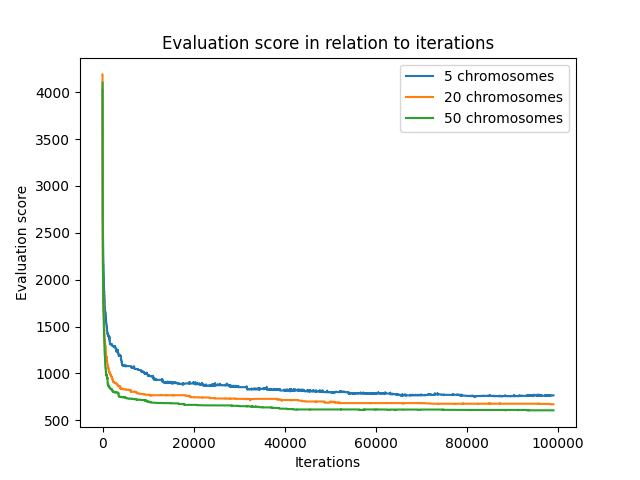
\includegraphics[scale=0.9]{img/131_no_inverse.png}
    \caption{Przebieg pierwszej wersji algorytmu dla grafu xqf131}
    \label{fig:131_no_inverse}
\end{figure}
Jak widać, algorytm bardzo szybko zbiega się do jakiegoś rozwiązania. Również
widać, że zwiększenie liczby osobników pozwala na odnalezienie lepszego
rozwiązania, dzięki rozważaniu większej ilości potencjalnych ścieżek.
Następnie ten sam algorytm został sprawdzony na większym grafie xqg237. Wyniki
są przedstawione na rysunku 
\begin{figure}[h]
    \centering
    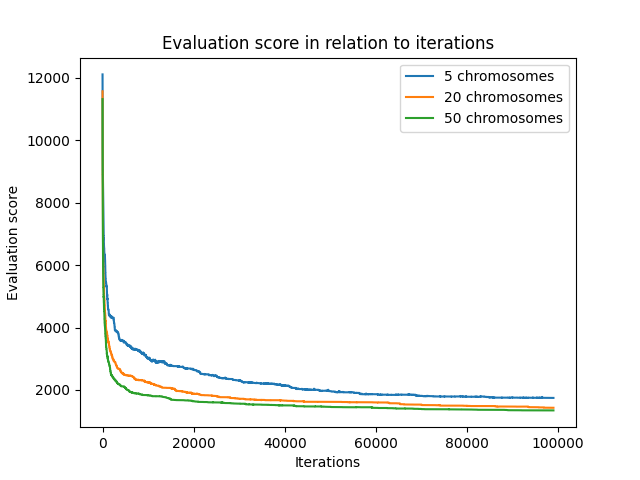
\includegraphics[scale=0.9]{img/237_no_inverse.png}
    \caption{Przebieg pierwszej wersji algorytmu dla grafu xqg237}
    \label{fig:237_no_inverse}
\end{figure}
Jest ta sama sytuacja jak w przypadku mniejszego grafu, rozwiązanie szybko się
zbiega, a większa liczba osobników pomaga znaleźć lepsze rozwiązanie.
Znalezione rozwiązania przedstawiono na rysunku \cref{fig:v1_solutions}
\begin{figure}
    \centerline{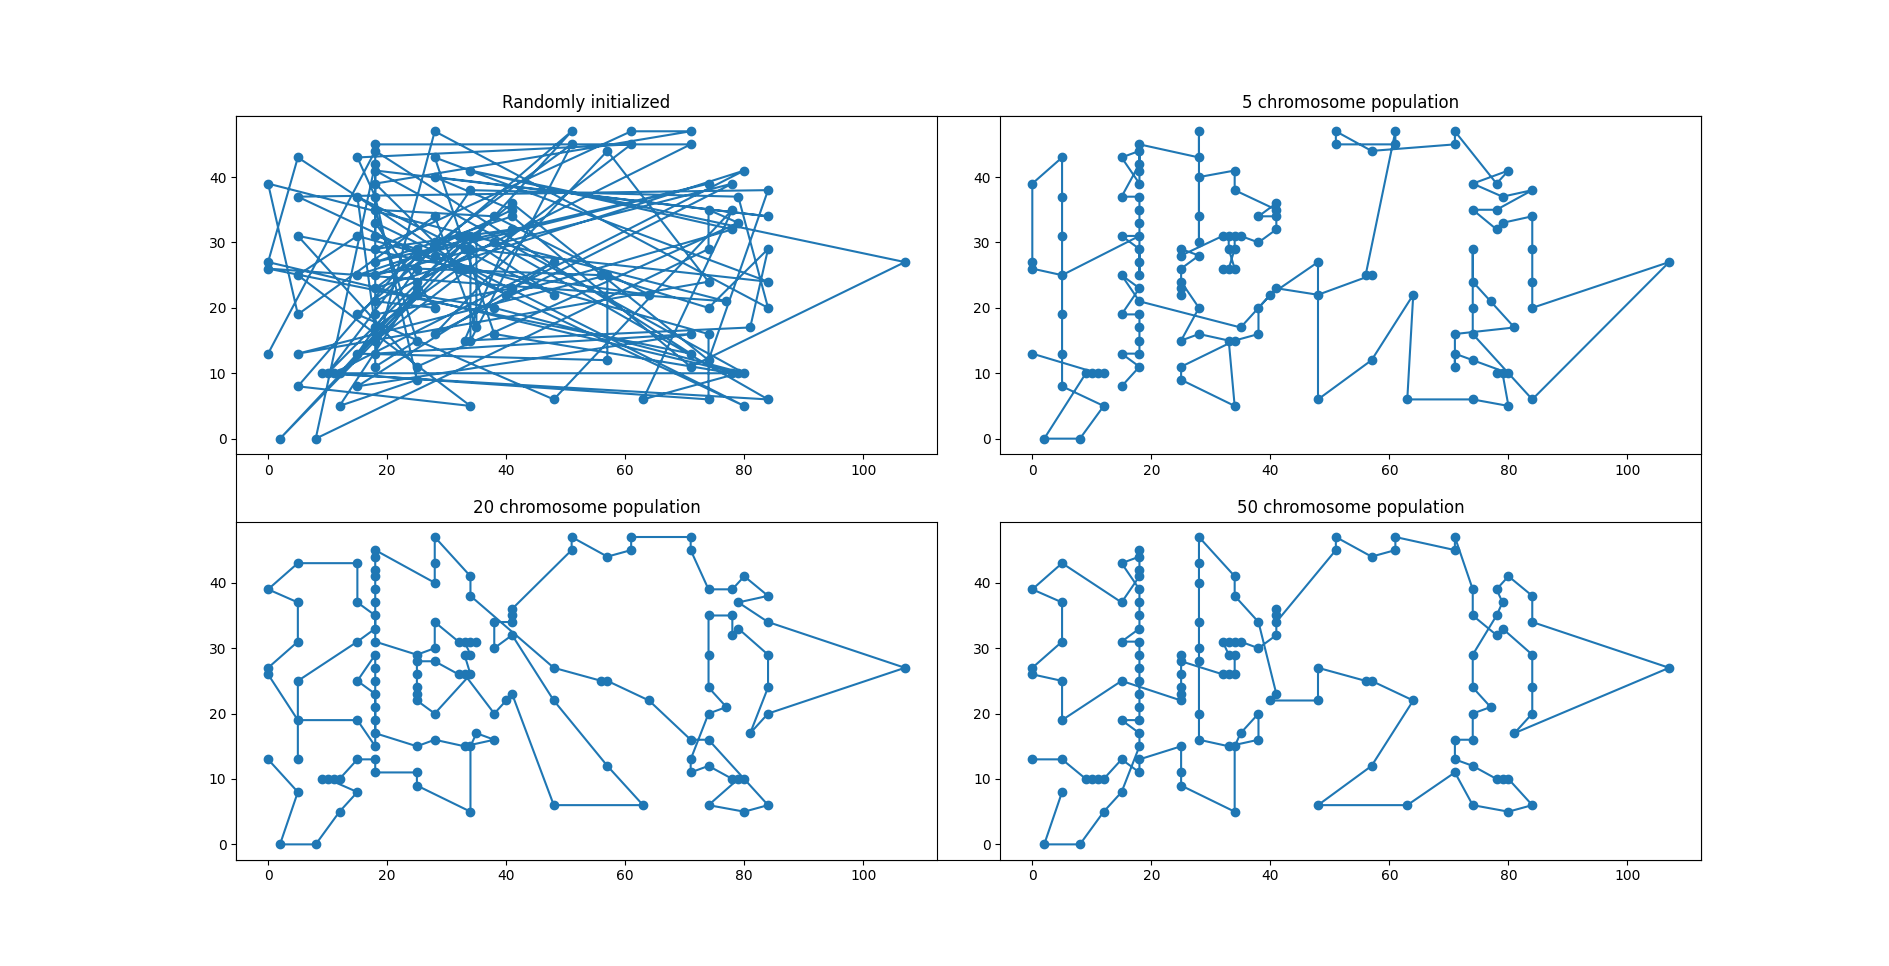
\includegraphics[scale=0.5]{../131_obrazy.png}}
    \caption{Znalezione rozwiązania grafu xqf131 dla poszczególnych populacji
    bez inwersji}
    \label{fig:v1_solutions}
\end{figure}
\begin{figure}
    \centerline{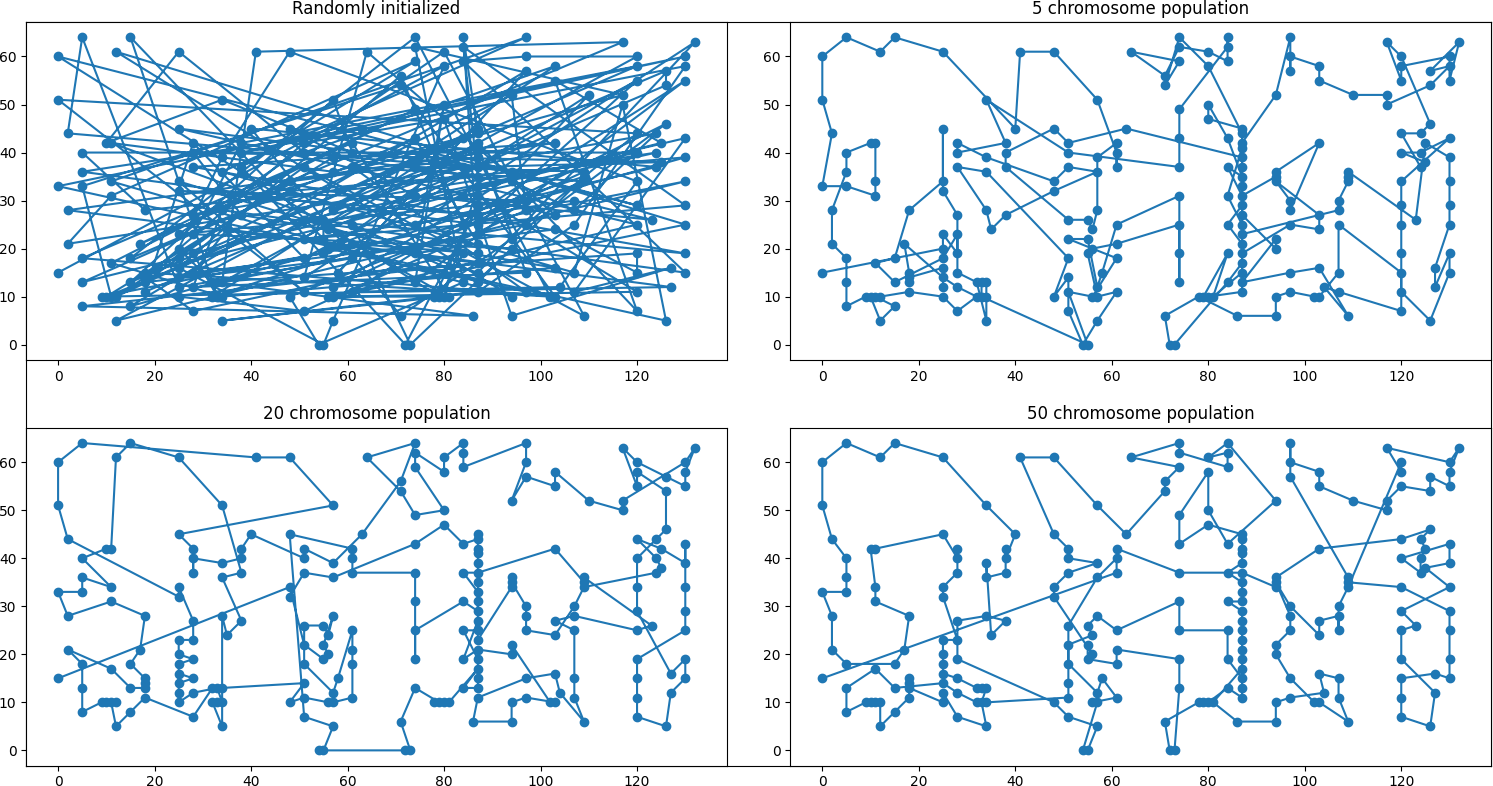
\includegraphics[scale=0.5]{../237_obrazy.png}}
    \caption{Znalezione rozwiązania grafu xqg237 dla poszczególnych populacji
    bez inwersji}
    \label{fig:v1_solutions_237}
\end{figure}

W kolejnej wersji programu, do mutacji została dodana inwersja, z myślą o tym,
aby ograniczyć wpadanie do minimum lokalnego. Wpływ tej modyfikacji jest
przedstawiony na rysunku \cref{fig:comparison}.
\begin{figure}
    \centering
    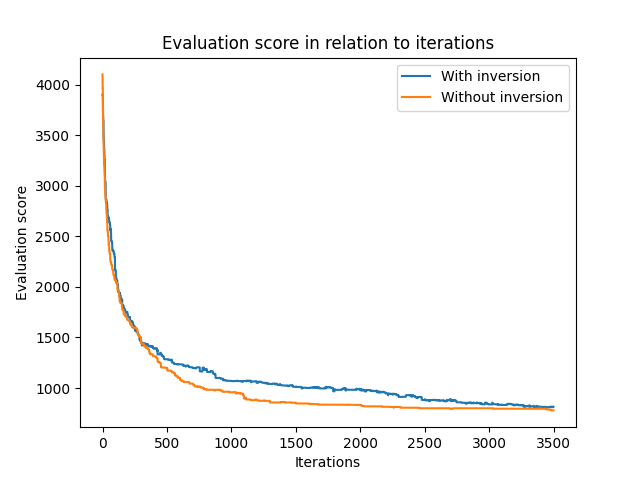
\includegraphics[scale=0.9]{img/comparison_50p_131.png}
    \caption{Porównanie dwóch wersji algorytmu dla grafu xqf131 i 50 osobników}
    \label{fig:comparison}
\end{figure}
Jak można zauważyć, dodanie inwersji faktycznie spowalnia zbieganie się
algorytmu, jednak ostatecznie rozwiązanie jest podobne.

Poza inwersją zostały użyte większe populacje. Przekłada się to na dłuższy czas
szukania rozwiązania, ale w zamian jest odszukane lepsze rozwiązanie. Na
rysunku \cref{fig:131_inverse} jest przedstawiony przebieg algorytmu po
modyfikacji dla grafu xqf131.
\begin{figure}[h]
    \centering
    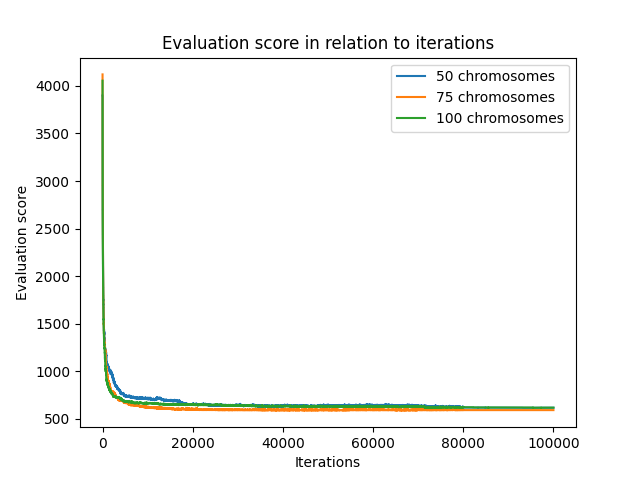
\includegraphics[scale=0.9]{img/131_inverse.png}
    \caption{Przebieg drugiej wersji algorytmu dla grafu xqf131}
    \label{fig:131_inverse}
\end{figure}
Algorytm dość szybko zbiega się do rozwiązania, pomimo dodania nowej mutacji,
ale jest to spowodowane większą ilością osobników. Samo rozwiązanie jest też
lepsze w porównaniu do poprzedniej wersji programu, bez inwersji.
Na rysunku \cref{fig:v2_solutions} przedstawiono znalezione ścieżki dla po
dodaniu inwersji do mutacji. Wyniki dla obu grafów są przedstawione w tebeli
\cref{tab1} oraz \cref{tab2}.
\begin{figure}
    \centerline{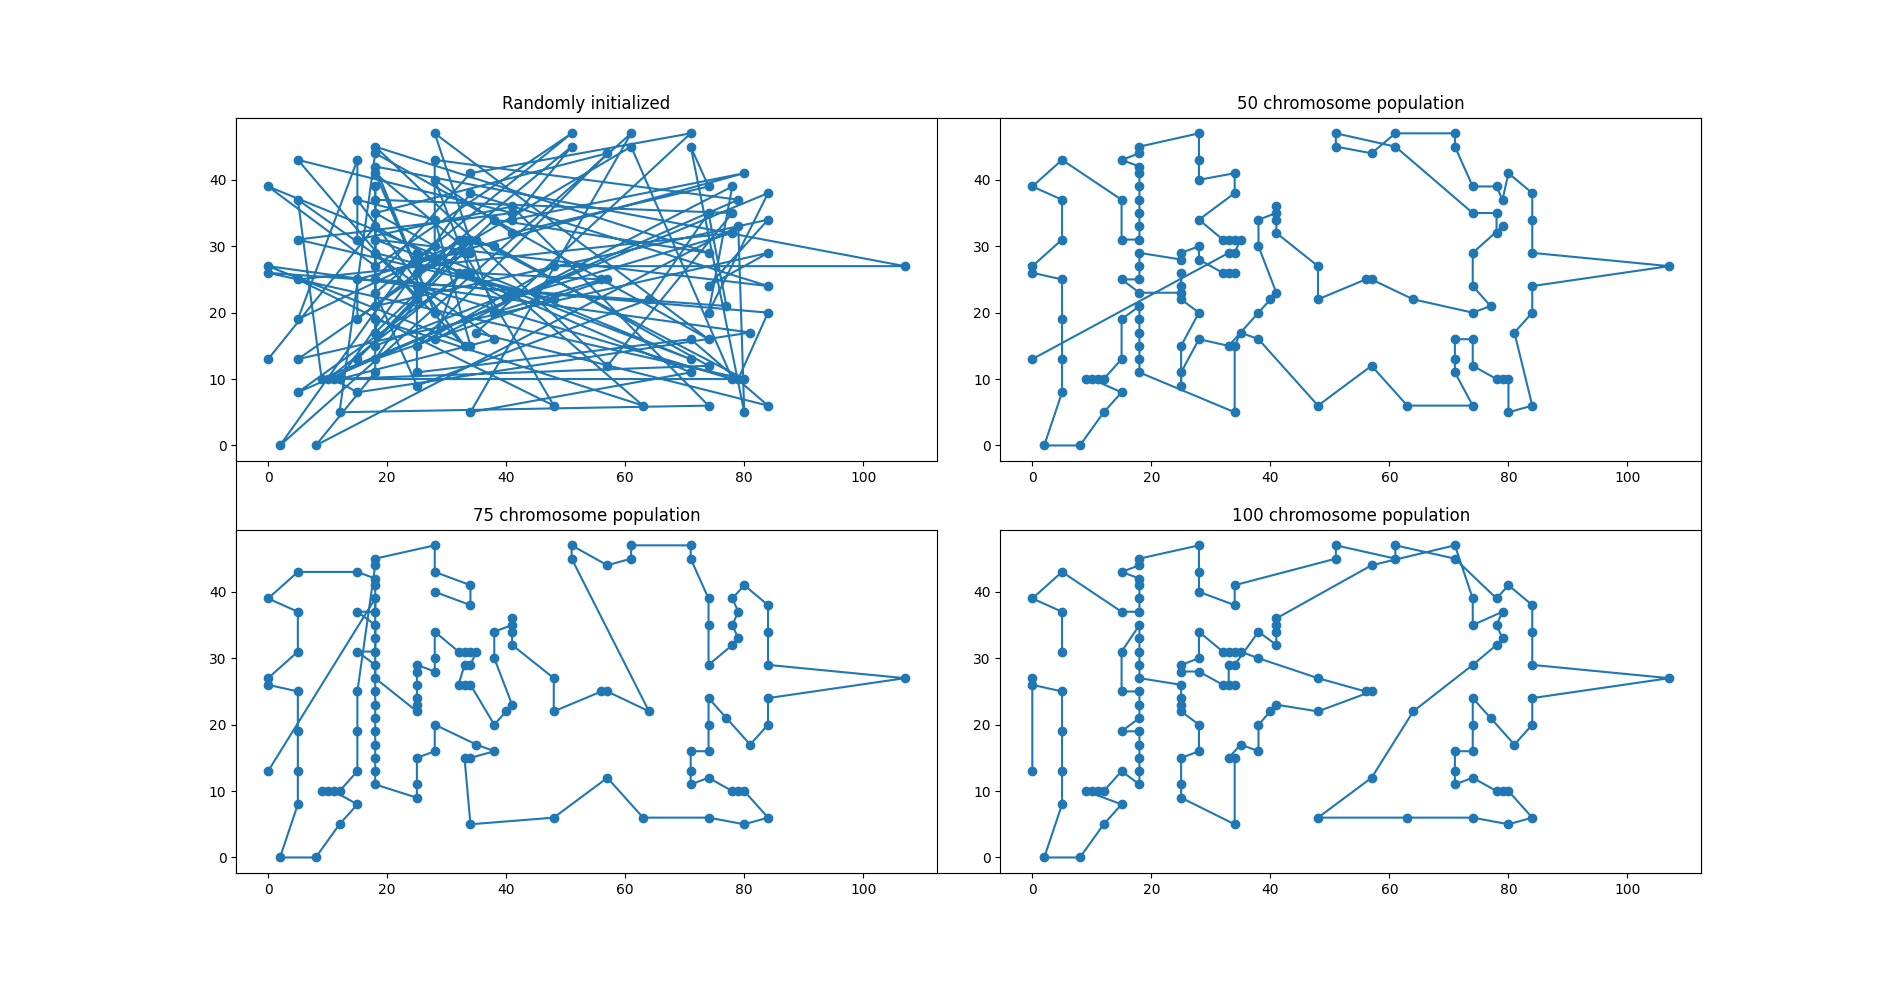
\includegraphics[scale=0.5]{../131_obrazy_inverse.png}}
    \caption{Znalezione rozwiązanie grafu xqf131 dla poszczególnych populacji po
    dodaniu inwersji}
    \label{fig:v2_solutions}
\end{figure}
\begin{table}[]
    \centering
    \begin{tabular}{|lll|}
    \hline
    \multicolumn{3}{|c|}{xqf131}                                            \\ \hline
    \multicolumn{1}{|l|}{populacja} & \multicolumn{1}{l|}{inwersja} & wynik \\ \hline
    \multicolumn{1}{|l|}{5}         & \multicolumn{1}{l|}{nie}      & 758   \\ \hline
    \multicolumn{1}{|l|}{20}        & \multicolumn{1}{l|}{nie}      & 670   \\ \hline
    \multicolumn{1}{|l|}{50}        & \multicolumn{1}{l|}{nie}      & 606   \\ \hline
    \multicolumn{1}{|l|}{50}        & \multicolumn{1}{l|}{tak}      & 615   \\ \hline
    \multicolumn{1}{|l|}{75}        & \multicolumn{1}{l|}{tak}      & 588   \\ \hline
    \multicolumn{1}{|l|}{100}       & \multicolumn{1}{l|}{tak}      & 614   \\ \hline
    \end{tabular}
    \caption{Otrzymane wyniki dla grafu xqf131 po $10^{6}$ iteracjach}
    \label{tab1}
\end{table}
\begin{table}[]
    \centering
    \begin{tabular}{|lll|}
    \hline
    \multicolumn{3}{|c|}{xqg237}                                            \\ \hline
    \multicolumn{1}{|l|}{populacja} & \multicolumn{1}{l|}{inwersja} & wynik \\ \hline
    \multicolumn{1}{|l|}{5}         & \multicolumn{1}{l|}{nie}      & 1744  \\ \hline
    \multicolumn{1}{|l|}{20}        & \multicolumn{1}{l|}{nie}      & 1428  \\ \hline
    \multicolumn{1}{|l|}{50}        & \multicolumn{1}{l|}{nie}      & 1344  \\ \hline
    \end{tabular}
    \caption{Otrzymane wyniki dla grafu xqg237 po $10^{6}$ iteracjach}
    \label{tab2}
\end{table}
\end{document}